% coding:utf-8

%----------------------------------------
%FOSAMATH, a LaTeX-Code for a mathematical summary for basic analysis
%Copyright (C) 2013, Daniel Winz, Ervin Mazlagic, Adrian Imboden, Philipp Langer

%This program is free software; you can redistribute it and/or
%modify it under the terms of the GNU General Public License
%as published by the Free Software Foundation; either version 2
%of the License, or (at your option) any later version.

%This program is distributed in the hope that it will be useful,
%but WITHOUT ANY WARRANTY; without even the implied warranty of
%MERCHANTABILITY or FITNESS FOR A PARTICULAR PURPOSE.  See the
%GNU General Public License for more details.
%----------------------------------------

% coding:utf-8
\section{Potenzreihe}
Ein Ausdruck der Form 
\[ \boxed{f(x) = \sum_{K = 0}^{\infty} a_K x^K 
= a_0 + a_1 x + a_2 x^2 + a_3 x^3 \dots a_K x^K} \]
wird Potenzreihe genannt. 
\[ \boxed{a_k = \frac{f^{(K)}(x_0)}{K!}} \]
$f^{(K)}(x)$ ist dabei die K-te Ableitung von $f(x)$ gemeint. 

\subsection{Taylorreihe mit Entwicklungspunkt $x_0 \neq 0$}
\[ \boxed{f(x) = \sum_{K=0}^{\infty}\frac{f^{(K)}(x_0)}{K!}\cdot (x-x_0)^K} \]
$f^{(K)}(x)$ ist dabei die K-te Ableitung von $f(x)$ gemeint. 
\[ \boxed{f(x) = \underbrace{\sum_{K=0}^{n}\frac{f^{(K)}(x_0)}
{K!} (x - x_0)^K}_{T_{(n,x_0)}(x)} + \underbrace{\sum_{K=n+1}^{\infty}
\frac{f^{(K)}(x_0)}{K!} (x - x_0)^K}_{R_{n+1}(x)}} \]
$T_{(n,x_0)}(x)$ ist dabei das Taylorpolynom vom Grad n und $R_{n+1}(x)$ ist 
das Restglied. \\
Für das Restglied gilt: Es gibt eine Zahl $\xi$ zwischen $x_0$ und $x$ so, dass 
gilt:
\[ \boxed{R_{n+1} = \frac{f^{(n + 1)}(\xi)}{(n + 1)!} \cdot (x - x_0)^{n + 1}}\]
Dies ist eine Restgliedformel (Lagrangsche Darstellung für $R_{n + 1}$).

\subsection{McLaurin-Reihe (Taylorreihe mit Entwicklungspunkt $x_0 = 0)$}
Eine Taylorreihe mit Entwicklungspunkt $x_0 = 0$ wird MacLaurin-Reihe genannt
\[ \boxed{f(x) = \underbrace{\sum_{K=0}^{\infty}
\frac{f^{(K)}(0)}{K!} x^K}_{\text{Taylorreihe}}} \]
$f^{(K)}(x)$ ist dabei die K-te Ableitung von $f(x)$ gemeint. 
\[ \boxed{f(x) = \underbrace{\sum_{K=0}^{n}
\frac{f^{(K)}(0)}{K!} x^K}_{T_{(n,x_0)}(x)} + 
\underbrace{\sum_{K=n+1}^{\infty}\frac{f^{(K)}(0)}{K!} x^K}_{R_{n+1}(x)}} \]
$T_{(n,x_0)}(x)$ ist dabei das Taylorpolynom vom Grad n und $R_{n+1}(x)$ ist 
das Restglied. \\
Für das Restglied gilt: Es gibt eine Zahl $\xi$ zwischen $x_0$ und $x$ so, dass 
gilt:
\[ \boxed{R_{n+1} = \frac{f^{(n + 1)}(\xi)}{(n + 1)!} \cdot (x - x_0)^{n + 1}}\]
Dies ist eine Restgliedformel (Lagrangsche Darstellung für $R_{n + 1}$).

\subsection{Konvergenzradius}
Der Konvergenzradius sagt aus, innerhalb von welchem Intervall (ausgehend vom 
Approximationspunkt)
eine Potenzreihe konvergiert. Der Begriff Radius ist dabei ein Skalar auf 
$\Omega$ und nicht im $\mathbb{R}^2$.

\begin{figure}[h!]
\centering
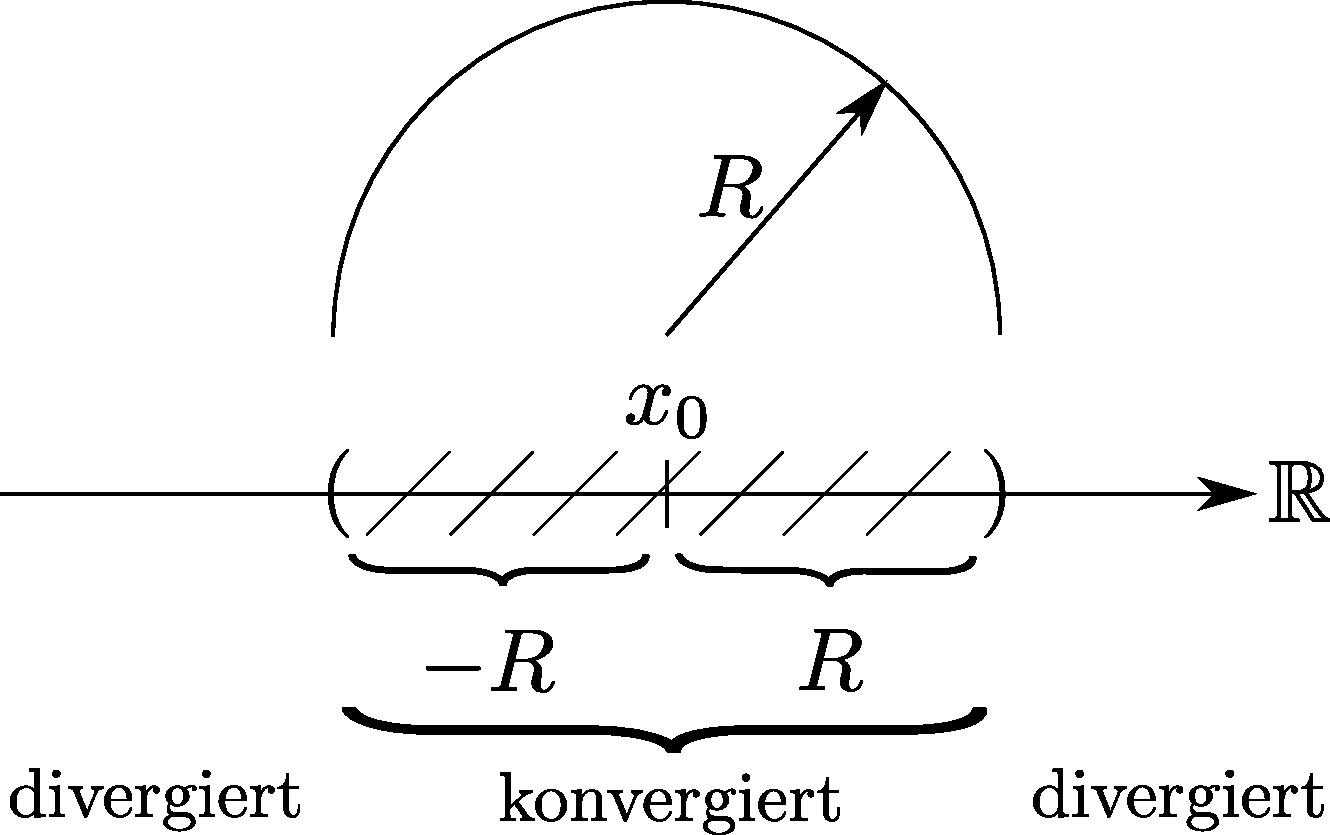
\includegraphics[width=0.6\textwidth]{konvergenzradius.pdf}
\end{figure}

\[ \boxed{ \begin{array}{lll} 
    |x| < R & \Rightarrow & \text{Potenzreihe ist konvergent} \\
    |x| > R & \Rightarrow & \text{Potenzreihe ist divergent} \\
    |x| = R & \Rightarrow & \text{überprüfen was für $x=R$ und $-x=R$ gilt}
\end{array} } \]

\[ \boxed{R = \frac{1}{q} = \lim_{K \rightarrow \infty} \left| 
\frac{a_K}{a_{K + 1}} \right|} \]
% \quad \quad \text{wobei} \quad \quad a_k = \frac{f^{(K)}(x_0)}{K!} } \]

\subsection{Einfache Funktionen als Taylorreihen}
\[ \boxed{e^x = \sum_{K=0}^{\infty} \frac{x^K}{K!}} \]
\[ \boxed{\sin(x) = \sum_{K=0}^{\infty} \frac{(-1)^K x^{2K+1}}{(2K+1)!}} \]
\[ \boxed{\cos(x) = \sum_{K=0}^{\infty} \frac{(-1)^K x^{2K}}{(2K)!}} \]
\[ \boxed{\cosh(x) = \sum_{K=0}^{\infty} \frac{x^{2K}}{(2K)!}} \]
\[ \boxed{\sinh(x) = \sum_{K=0}^{\infty} \frac{x^{2K+1}}{(2K+1)!}} \]

\subsection{Binomische Reihe}
\[ \boxed{(1 + x)^\alpha = \sum_{K=0}^{\infty}
\left(\begin{matrix}\alpha\\K\end{matrix}\right)x^k } \]
Den Ausdruck \( \left(\begin{matrix}N\\K\end{matrix}\right) \) nennt man 
Binomialkoeffizient. Man kann ihn folgendermassen berechnen:
\[ \boxed{\left(\begin{matrix}N\\K\end{matrix}\right) 
= \frac{N !}{K! \cdot (N - K)!}, N \in \mathbb{N}^{{}^{\ensuremath{\!+\!}}}_{}, 
K \in \mathbb{N}^{{}^{\ensuremath{\!+\!}}}_{} } \]

\iftiboth
\noindent
Berechnung mit dem Taschenrechner:
\begin{verbatim} ncr(N,K) \end{verbatim}
\fi

\noindent
Da für ganzzahlige positive Zahlen \( \frac{N !}{K! \cdot (N - K)!} \) gilt, 
gilt für ganzzahlige positive N auch folgendes:
\[ \boxed{(1 + x)^\alpha = \sum_{K=0}^{\infty}
\left(\begin{matrix}\alpha\\K\end{matrix}\right)x^k 
= \sum_{K=0}^{\infty}\frac{\alpha !}{K! \cdot (\alpha - K)!}x^k} \]

\subsection{Kochrezept Taylorreihen}
\begin{enumerate}
  \item Stelle finden, an welcher die Funktion approximiert werden soll. 
  \item Bereich und Genauigkeit bzw. Fehler definieren oder den Grad der 
  Potenzreihe fix wählen. 
  \item $a_0$, $a_1$, \dots $a_n$ berechnen. $n$ ist dabei der Grad der 
  Potenzreihe
  \item Potenzreihe zusammensetzten
\end{enumerate}

\ifti
\subsection{Taylorreihe mit dem TI-89 berechnen}
\begin{verbatim}
taylor(Funktion,Variable,Ordnung[,Punkt])
\end{verbatim}
Funktion: Funktion, zu welcher die Taylorreihe gesucht ist. \\
Variable: Variable in Funktion\\
Ordnung: Ordnung der Taylorreihe\\
Punkt: Optional: Punkt, an dem die Funktion approximiert wird. (Default: 0)
\fi
\ifnspire
\subsection{Taylorreihe mit dem TI-Nspire berechnen}
\begin{verbatim}
taylor(Funktion,Variable,Ordnung[,Punkt])
\end{verbatim}
Funktion: Funktion, zu welcher die Taylorreihe gesucht ist. \\
Variable: Variable in Funktion\\
Ordnung: Ordnung der Taylorreihe\\
Punkt: Optional: Punkt, an dem die Funktion approximiert wird. (Default: 0)
\fi
